%-------------------------------------------------------------------------------
%	PAQUETES Y OTRAS CONFIGURACIONES
%-------------------------------------------------------------------------------

%-------------------------------------------------------------------------------
%	PAQUETES Y OTRAS CONFIGURACIONES
%-------------------------------------------------------------------------------
\documentclass{tufte-handout}
%\documentclass[paper=letter, fontsize=11pt]{scrartcl} % Tamaño de papel y letra para el documento
\usepackage{geometry}
\geometry{left=1.2cm, right=6.2cm, top=2.5cm, bottom=2.5cm}
\usepackage{color}
\usepackage[utf8]{inputenc} % Los caracteres acentuados se pueden escribir normalmente en el código
\usepackage[T1]{fontenc} % Configuración de fuente de salida
\usepackage{cmbright}
\usepackage[sfdefault]{noto}
\usepackage[T1]{fontenc}
\normalfont
\usepackage{graphicx} % Paquetes para incluir imágenes
\usepackage{multicol}
\usepackage{circuitikz}
\usepackage{tikz}
\usetikzlibrary{arrows}

\usepackage{sectsty} % Paquete para configuración de secciones
\allsectionsfont{\centering \normalfont \scshape} % Los títulos de las secciones son centrados, con la misma fuente y pequeñas mayúsculas

\usepackage{todonotes}
\usepackage{microtype}
\renewcommand{\figurename}{Figura}

\usepackage{listings}
\renewcommand{\lstlistingname}{Código}
\lstdefinestyle{mystyle}{
    basicstyle=\footnotesize,
    breakatwhitespace=false,
    breaklines=true,
    captionpos=b,
    keepspaces=true,
    numbers=left,
    numbersep=5pt,
    showspaces=false,
    showstringspaces=false,
    showtabs=false,
    tabsize=2
}
\lstset{style=mystyle}

% \usepackage{fancyhdr} % Paquete para personalizar pies y cabeceras de página
% \pagestyle{fancyplain} % Todas las páginas con las mismas cabeceras y pies de página
% \fancyhead{} % Sin cabecera
% \fancyfoot[L]{} % Vacío en la izquierda del pie de página
% \fancyfoot[C]{} % Vacío en el centro del pie de página
% \fancyfoot[R]{\thepage} % Número de página en el pie de pagina
% \renewcommand{\headrulewidth}{0pt} % Sin lineas en la cabecera
% \renewcommand{\footrulewidth}{0pt} % Sin lineas en el pie de página
% \setlength{\headheight}{13.6pt} % Altura de cabecera
%
% \numberwithin{equation}{section} % Numera ecuaciones en cada sección
% \numberwithin{figure}{section} % Numera figuras en cada sección
% \numberwithin{table}{section} % Numera tablas en cada sección
%
% \setlength\parindent{0pt} % Quita la indentación de los párrafos

\newcommand{\horrule}[1]{\rule{\linewidth}{#1}} % Comando personalizado para hacer linea horizontal


%-------------------------------------------------------------------------------
%	TITULO
%-------------------------------------------------------------------------------

\title{Práctica 2 - Señales\\Interfaces y periféricos para robots}
\author{Roberto Cadena Vega} % Nombre del profesor
\date{}

%-------------------------------------------------------------------------------
%	EMPIEZA EL DOCUMENTO
%-------------------------------------------------------------------------------

\begin{document}
\maketitle % Imprime el título

%-------------------------------------------------------------------------------
%	OBJETIVOS
%-------------------------------------------------------------------------------

\section{Objetivos}

	Familiarizarse con los diferentes tipos de señales a manejarse para el control de sistemas automáticos.

%-------------------------------------------------------------------------------
%	CONOCIMIENTOS PREVIOS
%-------------------------------------------------------------------------------

\section{Conocimientos Previos}

%-------------------------------------------------------------------------------

	\subsection{Señales digitales}

		\begin{marginfigure}
			\begin{center}
				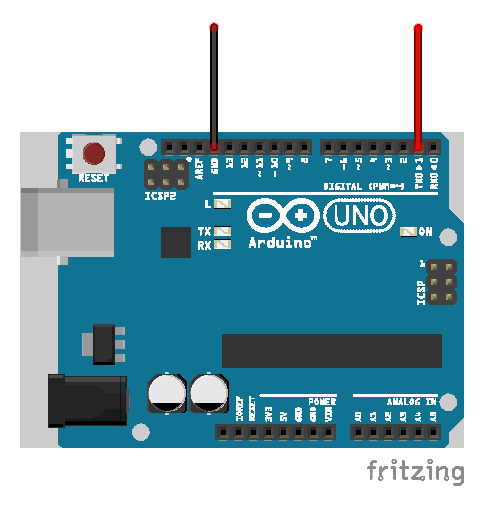
\includegraphics[width=\textwidth]{images/txosc.pdf}
				\caption{Conexion de Transmisión de datos del Arduino UNO}
				\label{fig:arduino-osc}
			\end{center}
		\end{marginfigure}

		Empezaremos esta práctica analizando la manera en que la tarjeta de desarrollo de Arduino transmite información a la computadora y viceversa.

		Las mediciones que se muestran se hicieron conectando la tarjeta de desarrollo de Arduino a un osciloscopio casero como se muestra en la figura \ref{fig:arduino-osc}, sin embargo tu tienes la oportunidad de seguir estas mediciones con un osciloscopio profesional pidiendo este equipo al personal de laboratorio, por lo que te sugiero que empieces con estas mediciones, antes de seguir con la parte importante de la práctica.

		Se empieza con el siguiente código cargado en la tarjeta de desarrollo:

		\lstinputlisting[language=C]{codigos/trans1.ino}

		En este código se inicializa el puerto serial con una tasa de transmisión de $9600 baudios$, se envía el dato $1$, seguido del terminador de linea (retorno de linea, enter) y espera $2ms$ para estabilizar el $\mu C$.

		\begin{marginfigure}
			\begin{center}
				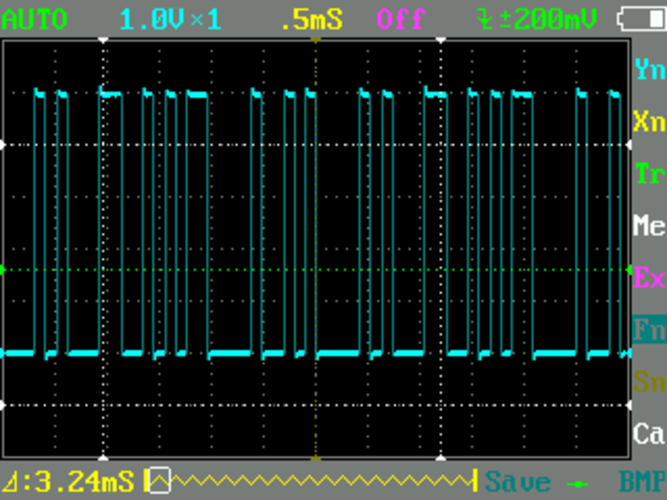
\includegraphics[width=\textwidth]{images/1ln2ms.pdf}
				\caption{Medición de transmisión de datos con $2ms$ de retraso}
				\label{fig:trans1}
			\end{center}
		\end{marginfigure}

		Sin embargo es dificil leer en donde empieza y en donde termina cada dato como se puede ver en la figura \ref{fig:trans1}, por lo que se modifica la ultima linea del código para que espere $10ms$ el $\mu C$ como se ve en la figura \ref{fig:trans2}.

		\begin{marginfigure}
			\begin{center}
				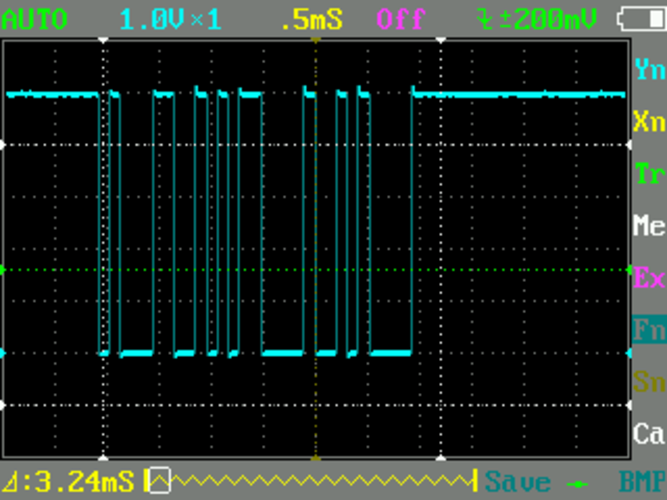
\includegraphics[width=\textwidth]{images/1ln10ms.pdf}
				\caption{Medición de transmisión de datos con $10ms$ de retraso}
				\label{fig:trans2}
			\end{center}
		\end{marginfigure}

		Aún en esta figura estamos viendo mas bits de los que realmente queremos medir, por lo que cambiaremos la instrucción \texttt{println} por \texttt{print} para que solo envíe el dato que queremos, sin el terminador de linea, y podemos ver en la figura \ref{fig:trans3} que la transmisión en realidad consiste de $9$ bits. Tambien podemos notar que el estado de descanso de la transmisión de datos es $5V$, por lo que si analizamos esta transmisión de datos desde el punto de vista de la computadora, si mandamos un dato que empiece con un $1$ lógico, la computadora no tendría manera de saber que empezamos a mandar el dato; es necesario que mandemos un $0$ lógico siempre que mandemos un dato, no importa cual sea el dato.

		Tomando en cuenta esto, y que la transmisión de datos empieza con el bit menos significativo, tenemos que esta señal, la podemos decodificar como el siguiente byte:

		\begin{equation}
			 \underbracket{0011}_{\mathclap{\text{Nibble mayor}}} \overbracket{0001}^{\mathclap{\text{Nibble menor}}} = 49_{10}
		\end{equation}

		\begin{figure}
			\begin{center}
				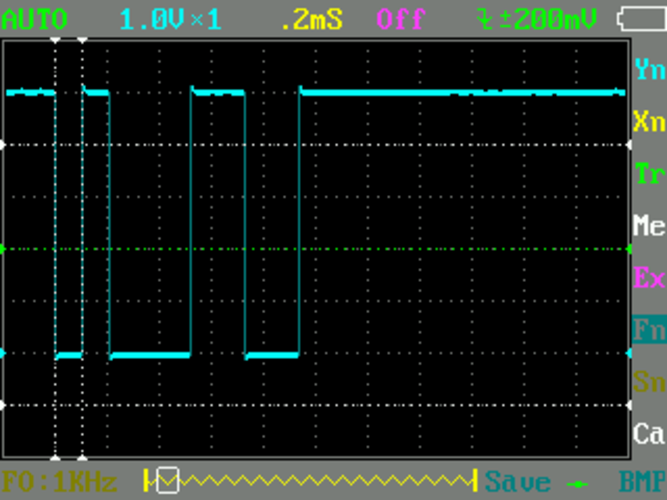
\includegraphics[width=0.5\textwidth]{images/110msz.pdf}
				\caption{Transmisión de dato $1$}
				\label{fig:trans3}
			\end{center}
		\end{figure}

		Lo cual obviamente no es el dato $1$, sin embargo, si nos fijamos en la tabla de caracteres ASCII, podemos ver que $49$ corresponde al caracter "1".

		Si ahora modificamos el código para enviar el dato "1", en lugar del dato $1$, nos damos cuenta que en efecto, el $\mu C$ esta convirtiendo $1$ en caracter y despues enviandolo.

		Podemos hacer una prueba más, cambiando "1" por "a", con lo que obtendremos la transmisión de la figura \ref{fig:trans4}.

		\begin{marginfigure}
			\begin{center}
				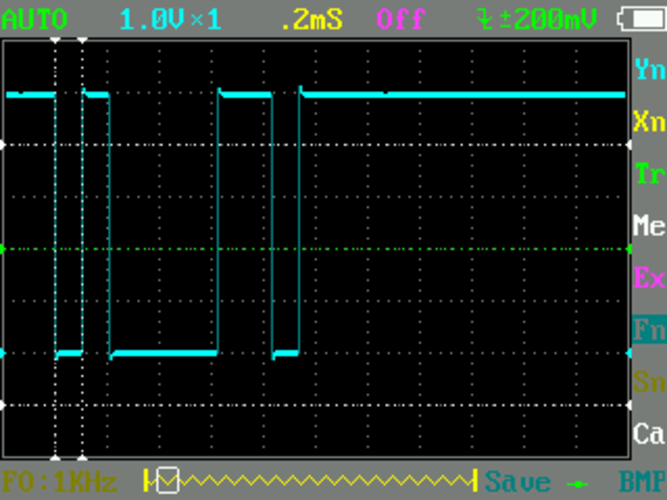
\includegraphics[width=\textwidth]{images/a10msz.pdf}
				\caption{Transmisión de dato "a"}
				\label{fig:trans4}
			\end{center}
		\end{marginfigure}

		Notemos que estos datos que hemos enviado, no solo se pueden interceptar por medio del pin \texttt{Tx}, mas bien, estos datos tienen la intención de llegar a la computadora por medio de la conversión de datos del chip FTDI o bien CH340G y al puerto serial de la computadora.

		Podemos darnos cuenta de esto si abrimos el monitor serial del IDE de Arduino (Menú principal, Herramientas, Monitor Serie), podremos ver una pantalla como la de la figura \ref{fig:mon-ser}.

		\begin{figure}
			\begin{center}
				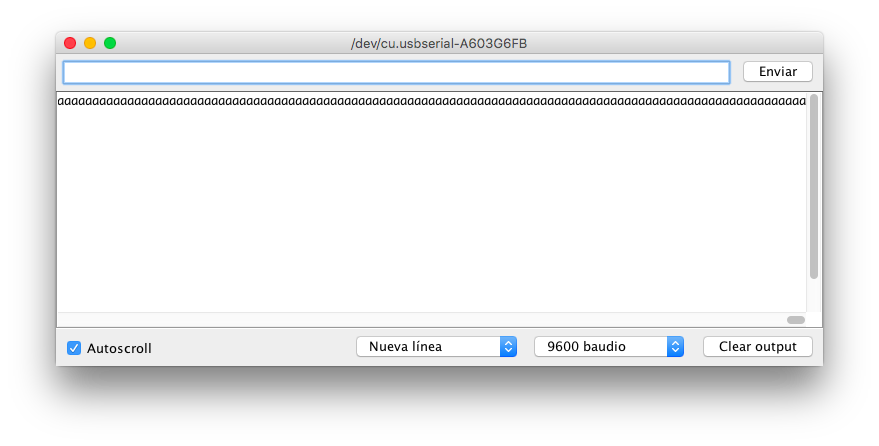
\includegraphics[width=\textwidth]{images/monitor-serial.png}
				\caption{Monitor serial del IDE de Arduino}
				\label{fig:mon-ser}
			\end{center}
		\end{figure}

		%\newpage

%-------------------------------------------------------------------------------
%	EQUIPO
%-------------------------------------------------------------------------------

\section{Equipo}

	El siguiente equipo será proporcionado por el laboratorio, siempre y cuando lleguen en los primeros 15 minutos de la práctica, y hagan el vale conteniendo el siguiente equipo (exceptuando las pinzas).

	\begin{itemize}
		\item Osciloscopio
		\item Cables BNC - Caimán
		\item Cable de alimentación
		\item Multímetro
		\item Pinzas
	\end{itemize}

%-------------------------------------------------------------------------------
%	MATERIALES
%-------------------------------------------------------------------------------

\section{Materiales}

	\begin{itemize}
		\item Protoboard
		\item Potenciometro ($1k\Omega$, $10k\Omega$, etc.)
		\item Cables
	\end{itemize}

%-------------------------------------------------------------------------------
%	DESARROLLO
%-------------------------------------------------------------------------------

\section{Desarrollo}

	Para el desarrollo de esta práctica es necesario que cargues el siguiente programa a tu tarjeta de desarrollo Arduino:

	\lstinputlisting[language=C]{codigos/trans_anal.ino}

	Diseña un circuito de tal manera que el arduino lea la resistencia variable de un potenciometro.

%-------------------------------------------------------------------------------
%	CONCLUSIONES
%-------------------------------------------------------------------------------

\section{Conclusiones}
	El alumno deberá describir sus conclusiones al final de su reporte de práctica.

%-------------------------------------------------------------------------------
%	HOJA DE ANOTACIONES
%-------------------------------------------------------------------------------

\clearpage
\section{Hoja de Anotaciones}

	\begin{enumerate}
		\item ¿Cuál es el tiempo de estabilización del voltaje de salida cuando cambia de $0V$ a $5V$? \\ \vspace{0.9cm}

		\item ¿Cuál es el tiempo de estabilización del voltaje de salida cuando cambia de $5V$ a $0V$? \\ \vspace{0.9cm}

		\item Tomando en cuenta que el Arduino esta configurado para $9600 baudios$ ¿Que tiempo teórico debe tomar la transmisión de un bit de información? \\ \vspace{0.9cm}

		\item Tomando en cuenta que el Arduino esta configurado para $9600 baudios$ ¿Que tiempo real toma la transmisión de un bit de información? \\ \vspace{0.9cm}

		\item Tomando en cuenta que el Arduino esta configurado para $9600 baudios$ ¿Que tiempo real toma la transmisión de un caracter de información? \\ \vspace{0.9cm}

		\item ¿Cuantos bits son transmitidos, si se envía el dato $1$? ¿Porqué? \\ \vspace{0.9cm}

		\item ¿Cuantos bits son transmitidos, si se envía el dato $1.0$? ¿Porqué? \\ \vspace{0.9cm}

		\item Diseña el código de Arduino que envie los caracteres "bola" a la computadora, cada que la computadora le envie los caracteres "hola".

		\item ¿Que tiempo toma la transmisión de estos datos en teoría? ¿En realidad? \\ \vspace{0.9cm}

		\item Diseña el circuito necesario para que el código descrito en el desarrollo lea la posición de un potenciometro. Utiliza la parte posterior de esta hoja.

		\item Utiliza el multimetro, el osciloscopio y la grafica serial del IDE de Arduino para medir los niveles de voltaje en el potenciometro; caracteriza la señal obtenida por el multimetro, por el osciloscopio y la grafica del IDE en una grafica en la parte posterior de esta hoja.

		\item Carga el ejemplo Fading que se utilizó en la práctica 1, utiliza un multimetro y un osciloscopio para caracterizar la señal dada al LED.
	\end{enumerate}

	\begin{multicols}{2}
		Integrantes del equipo: \\[0.4cm]
		\horrule{0.5pt} \\[0.4cm] % Linea horizontal delgada
		\horrule{0.5pt} % Linea horizontal delgada

		Revisó: \\[1.25cm]
		\horrule{0.5pt} \\% Linea horizontal delgada
	\end{multicols}

%-------------------------------------------------------------------------------
%	FIN DEL DOCUMENTO
%-------------------------------------------------------------------------------

\end{document}
